\documentclass[a4paper,12pt,russian]{extreport}

\usepackage[14pt]{extsizes} %чтобы был 14-й шрифт		
\usepackage{polyglossia}   %% загружает пакет многоязыковой вёрстки
\setdefaultlanguage{russian}  %% устанавливает главный язык документа
\setotherlanguage{english} %% объявляет второй язык документа
\defaultfontfeatures{Ligatures={TeX}}  %% свойства шрифтов по умолчанию
\setmainfont[Ligatures={TeX,Historic}]{Times New Roman} %% задаёт основной шрифт документа
\setsansfont{Arial}                    %% задаёт шрифт без засечек
\setmonofont{Courier New}               %% задаёт моноширинный шрифт
\newfontfamily{\cyrillicfonttt}{Courier New} % моноширинный шрифт, на который не ругается компилятор
\usepackage{cmap}

%%%%%%%%%%%%%%%%%%%%%%%Images
\usepackage{graphicx}
\graphicspath{{images/}} 	%Папка куда надо складывать фото относительно root
\usepackage{epstopdf} 		%Для конвертации eps фото в pdf в includegraphics
%%%%%%%%%%%%%%%%%%%%%%%Images

\usepackage{amsmath, amsthm, amsfonts}
\usepackage{indentfirst}
\usepackage[usenames,dvipsnames]{color}
\usepackage[table,xcdraw]{xcolor}
\usepackage{makecell}
\usepackage{multirow}
\usepackage{float} %for absolute positioning of photos and etc.
\usepackage{ulem}
\usepackage{tocloft}
\usepackage{import}
\usepackage{lastpage}
\usepackage{etoolbox}
\usepackage[title,titletoc]{appendix}
\usepackage{pdfpages}

%%%%%%%%%%%%%%%%%%%%%%%Listings%%%%%%%%%%%%%%%%%%%%%%%%%%

\usepackage{color}
\definecolor{deepblue}{rgb}{0,0,0.5}
\definecolor{deepred}{rgb}{0.6,0,0}
\definecolor{deepgreen}{rgb}{0,0.4,0}
\definecolor{mygreen}{RGB}{28,172,0} % color values Red, Green, Blue
\definecolor{mylilas}{RGB}{170,55,241}

\usepackage{listings}

\lstset{
	language=Python,
	otherkeywords={self},   % Any extra options here
	keywordstyle=\color{deepred},
	showstringspaces=false,
	stringstyle=\color{deepgreen},
	%frame=tb,   %frame
	commentstyle=\color{deepgreen}
}

\lstset{language=Matlab,
	%breaklines=true,%
	morekeywords={matlab2tikz},
	keywordstyle=\color{blue},%
	identifierstyle=\color{black},%
	stringstyle=\color{mylilas},
	commentstyle=\color{mygreen},%
	showstringspaces=false,%without this there will be a symbol in the places where there is a space
	numbers=left,%
	numbersep=9pt % this defines how far the numbers are from the text
}

%%%%%%%%%%%%%%%%%%%%%%%Listings%%%%%%%%%%%%%%%%%%%%%%%%%%

\usepackage{todonotes}
\usepackage{xr}
\usepackage{dsfont}
\usepackage{algorithm2e}

\usepackage[font=it]{caption}
\usepackage{fancyhdr}
%\pagestyle{fancy}
%\fancyhf{}
%\fancyhead[R]{\thepage}
%\fancyheadoffset{0mm}
%\fancyfootoffset{0mm}
\setlength{\headheight}{17pt}
\renewcommand{\headrulewidth}{0pt}
\renewcommand{\footrulewidth}{0pt}
%\fancypagestyle{plain}{
%	\fancyhf{}
%	\rhead{\thepage}}
%\setcounter{page}{5}

\linespread{1.3}
\frenchspacing

%%% to allow custom headings
\usepackage{titlesec}
% to change titles font family
\usepackage{titling}

\titleformat{\chapter}[display]
	{\filcenter}
	{\MakeUppercase{\chaptertitlename} \thechapter}
	{8pt}
	{\bfseries}{}
	
\titleformat{\paragraph}[display]
	{\filcenter}
	{\MakeUppercase{\chaptertitlename} \thechapter}
	{8pt}
	{\bfseries}{}
	
\titleformat{\section}
	{\normalsize\bfseries}
	{\thesection}
	{1em}{}

\titleformat{\subsection}
	{\normalsize\bfseries}
	{\thesubsection}
	{1em}{}
	
\titlespacing*{\chapter}{0pt}{-30pt}{8pt}
\titlespacing*{\paragraph}{0pt}{-30pt}{8pt}
\titlespacing*{\section}{\parindent}{*4}{*4}
\titlespacing*{\subsection}{\parindent}{*4}{*4}

\renewcommand{\cfttoctitlefont}{\hspace{0.38\textwidth} \bfseries\MakeUppercase}
\renewcommand{\cftbeforetoctitleskip}{-1em}
\renewcommand{\cftaftertoctitle}{\mbox{}\hfill \\ \mbox{}\hfill{\footnotesize Стр.}\vspace{-2.5em}}
\renewcommand{\cftchapfont}{\normalsize\bfseries \MakeUppercase{\chaptername} }
\renewcommand{\cftsecfont}{\hspace{31pt}}
\renewcommand{\cftsubsecfont}{\hspace{11pt}}
\renewcommand{\cftbeforechapskip}{1em}
\renewcommand{\cftparskip}{-1mm}
\renewcommand{\cftdotsep}{1}
\setcounter{tocdepth}{2}
\setcounter{secnumdepth}{5}

\usepackage[square, numbers, sort&compress]{natbib}

\makeatletter
\renewcommand{\@dotsep}{2}
\newcommand{\l@likechapter}[2]{{\bfseries\@dottedtocline{0}{0pt}{0pt}{#1}{#2}}}

\newcommand{\likechapterheading}[1]{
	\begin{center}
	\textbf{\MakeUppercase{#1}}
	\end{center}
	\empline}
\newcommand{\likechapter}[1]{	
	\phantomsection
	\likechapterheading{#1}	
	\addcontentsline{toc}{likechapter}{\texorpdfstring{\MakeUppercase{#1}}{#1}}}


%%%%%%%%%%%%%%%Список литературы
\newcommand{\empline}{\mbox{}\newline}
\renewcommand{\bibnumfmt}[1]{#1.\hfill}
%\renewcommand{\bibnumfmt}[1]{[#1]\hfill}
\renewcommand{\bibsection}{\likechapter{Список литературы}}
\setlength{\bibsep}{0pt}
%%%%%%%%%%%%%%%Список литературы

\newcommand{\append}[1]{
	\clearpage
	\stepcounter{chapter}	
	\paragraph{\MakeUppercase{#1}}
	\empline
	\addcontentsline{toc}{likechapter}{\texorpdfstring{\chaptertitlename~\Asbuk{chapter}\;#1}}{\chaptertitlename~\Asbuk{chapter}:~#1}}
	
\usepackage{geometry}
\geometry{left=25mm}
\geometry{right=10mm}
\geometry{top=20mm}
\geometry{bottom=20mm}

%Таблицы и рисунки (формат подписи)
\usepackage[tableposition=top]{caption}
\usepackage{subcaption}
\DeclareCaptionLabelFormat{gostfigure}{Рисунок #2}
\DeclareCaptionLabelFormat{gosttable}{Таблица #2}
\DeclareCaptionLabelSeparator{gost}{~---~}
\captionsetup{labelsep=gost}
\captionsetup[figure]{labelformat=gostfigure}
\captionsetup[table]{labelformat=gosttable}
\renewcommand{\thesubfigure}{\asbuk{subfigure}}

\usepackage[xetex,bookmarks=true,colorlinks=true,linkcolor=blue,citecolor=Green,linktoc=none]{hyperref} 
\newcommand{\term}[1]{\textit{#1}}
\newcommand{\bydef}{\ensuremath{\stackrel{\text{\upshape df}}{=}}}
\newcommand{\<}{\langle}
\renewcommand{\>}{\rangle}
\newcommand{\includechapter}[1]{\subimport{chapter_#1/}{chapter_#1}}

\newtheorem{theorem}{Теорема}
\newtheoremstyle{break}
  {\topsep}{\topsep}%
  {\itshape}{}%
  {\bfseries}{}%
  {\newline}{}%
\theoremstyle{break}

\newtheorem{definition}{Определение}
\newtheorem{corollary*}{Следствие}
\newtheorem{lemma}{Лемма}

\newcommand{\condset}[2]{\braces{\, #1 \mid #2 \,}}
\newcommand{\walls}[1]{\left | #1 \right |} 
\newcommand{\norm}[2]{\left{||}#1\right{||}_{#2}} 
\newcommand{\set}[1]{\left\{ #1 \right\}}
\newcommand{\inprod}[3]{\left < #1,#2\right >_#3}

\newcommand{\HRule}{\rule{\linewidth}{0.5mm}}

\begin{document}
\vbox to \textheight{\renewcommand{\baselinestretch}{1}\selectfont%чтобы не было 1.5 интервала в заголовке
	\thispagestyle{empty} 
	\begin{center}
		\normalsize{\sffamily МИНОБРНАУКИ РОССИИ}\\
		{ \sffamily \mbox{\small{\textbf{ФЕДЕРАЛЬНОЕ ГОСУДАРСТВЕННОЕ БЮДЖЕТНОЕ ОБРАЗОВАТЕЛЬНОЕ УЧРЕЖДЕНИЕ}}} }\\ 
		{\sffamily \small{\textbf{ВЫСШЕГО ОБРАЗОВАНИЯ}} }\\
		\normalsize{\textbf{ \sffamily \textquotedblleft SUSPENDISSE VENENATIS\textquotedblright}}\\
		\vspace{0.2cm} 
		\normalsize{\sffamily Факультет \textit{nullam vitae}}\\
		%\vspace{0.01cm} 
		\normalsize{\sffamily Кафедра \textit{pellentesque sed}}\\
		\vspace{2.5cm}
		\normalsize{\textit{\sffamily Lorem ipsum dolor sit amet}}\\
		\vspace{2.5cm}
		\normalsize{\sffamily ВКР \textit{Магистерская диссертация}\\
			\vspace{0.5cm}
			{\sffamily \textit{01.01.01 Etiam mattis malesuada velit ut ultrices}}\\
			\vspace{0.5cm}
			{\sffamily \textit{Pellentesque euismod leo eget sem molestie ultricies}} }\\
		\vspace{4cm}

		{\sffamily%
			\begin{tabular}{lll}
				\multicolumn{3}{l}{Допущено к защите в ГЭК}  \\\\
				Зав.кафедрой &  \underline{\hspace{2cm}}  &\textit{A. A. Curabitur, д.ф.-м.н., профессор} \underline{\hspace{0.5cm}}.\underline{\hspace{0.5cm}}.20\underline{\hspace{0.5cm}}  \\\\
				Обучающийся & \underline{\hspace{2cm}} & \textit{N. V. Mauris, 2 курс, д/о } \\\\
				Руководитель & \underline{\hspace{2cm}} & \textit{I. F. Vestibulum, к.ф.-м.н., доцент}
			\end{tabular}
		}
		
	\end{center}
	
	\vspace{3.0cm}
	\vfill
	\vfill
	\begin{center}
		{\sffamily
			Athens 2018}
	\end{center}
}
\eject
\vbox to \textheight{\renewcommand{\baselinestretch}{1}\selectfont%чтобы не было 1.5 интервала в заголовке
	\thispagestyle{empty}
	\begin{center}
		\normalsize{\sffamily МИНОБРНАУКИ РОССИИ}\\
		{ \sffamily \mbox{\small{\textbf{ФЕДЕРАЛЬНОЕ ГОСУДАРСТВЕННОЕ БЮДЖЕТНОЕ ОБРАЗОВАТЕЛЬНОЕ УЧРЕЖДЕНИЕ}}} }\\ 
		{\sffamily \small{\textbf{ВЫСШЕГО ОБРАЗОВАНИЯ}} }\\
		\vspace{0.2cm}
		\normalsize{\textbf{ \sffamily <<SUSPENDISSE VENENATIS>>}}\\
		\normalsize{\textbf{ \sffamily(ФГБОУ ВО <<SV>>)}}\\
		\vspace{0.2cm} 
		\normalsize{\sffamily Факультет nullam vitae}\\
		%\vspace{0.01cm} 
		\normalsize{\sffamily Кафедра pellentesque sed}\\
	\end{center}
		
		%\vspace{1.5cm}
   \begin{flushright} 
   	   {\sffamily
			УТВЕРЖДАЮ\\
			заведующий кафедрой\\
			\underline{\hspace{3.0cm} Curabitur A. A.} \\
			{\footnotesize  \textit{подпись, расшифровка подписи}}\\
			\underline{\hspace{1.0cm}}.\underline{\hspace{1.0cm}}.20\underline{\hspace{0.5cm}}
		}
   \end{flushright}
   \begin{center}
   	{\sffamily
		\textbf{ЗАДАНИЕ}\\
		\textbf{\mbox{НА ВЫПОЛНЕНИЕ ВЫПУСКНОЙ КВАЛИФИКАЦИОННОЙ РАБОТЫ}}\\
		\textbf{ОБУЧАЮЩЕГОСЯ} $\underset{\text{\textit{фамилия, имя, отчество}}}{\text{\textbf{\underline{MAURIS NUNC VESTIBULUM}}}}$ }\\
     \end{center}	
   \begin{flushleft}
    {\small \sffamily
		1. Тема работы \textit{\underline{Lorem ipsum dolor sit amet}}, утверждена решением учёного совета 
		\underline{\hspace{2.0cm}} факультета от \underline{\hspace{1.0cm}}.\underline{\hspace{1.0cm}}.20\underline{\hspace{0.5cm}}\\
		2. Направление подготовки $\underset{\text{\textit{шифр, наименование}}}{\text{\underline{\textit{01.01.01 Etiam mattis malesuada velit ut ultrices}}}}$\\
		3. Срок сдачи законченной работы \underline{\hspace{1.0cm}}.\underline{\hspace{1.0cm}}.20\underline{\hspace{0.5cm}}\\
		4. Календарный план: (строится в соответствии со структурой ВКР)
	}
	\end{flushleft}
   \begin{flushleft}
   	{\sffamily \small
		\begin{tabular}{|m{0.4cm}|m{8.0cm}|m{4.0cm}|m{3.0cm}|}
				  \hline
				№ & Структура ВКР & Сроки выполнения & Примечание \\
				  \hline
				  & Lorem & \textbf{02.10.15 - 16.10.15} & \\
				  \hline
	\textbf{1} & Ipsum  & \textbf{16.10.15 - 25.12.15} & \\
				  \hline
	\textbf{2}  & Dolor  & \textbf{25.12.15 - 29.04.16} & \\
			      \hline
	\textbf{3}  & Sit  & \textbf{29.04.16 - 06.05.16} & \\
			      \hline
			     & Amet & \textbf{06.05.16 - 13.05.16} & \\
			      \hline
		\end{tabular}
	}
\end{flushleft}
	\begin{flushleft}
		{ \sffamily
		\begin{tabular}{llc}
			Обучающийся & \hspace{1.0cm} $\underset{\text{\textit{Подпись}}}{\text{\underline{\hspace{5.5cm}}}}$  \hspace{1.0cm} & $\underset{\text{\textit{расшифровка подписи}}}{\text{Mauris N. V.}}$ \\\\
			Руководитель & \hspace{1.0cm} $\underset{\text{\textit{Подпись}}}{\text{\underline{\hspace{5.5cm}}}}$ \hspace{1.0cm} & $\underset{\text{\textit{расшифровка подписи}}}{\text{Vestibulum I. F.}}$\\
		\end{tabular}
	    }
	\end{flushleft}
}
\eject
\clearpage

%\thispagestyle{empty} %убрали номер страницы
%%%%%%%%%%%%%%%%%%%%%%%%%Страница реферат%%%%%%%%%%%%%%%%%%%%%%%%%%%%%%%
\likechapterheading{Реферат}
Отчёт \pageref*{LastPage}~с., NNN~табл., NNN~рис.,  NNN~источ., NNN~прил.
~\\
~\\
LOREM, IPSUM, DOLOR, SIT, AMET

Объект исследования: Lorem ipsum dolor sit amet, consectetur adipiscing elit. Nam ut molestie magna. Mauris lacus ante, ullamcorper et dui eu, porta mattis nisl. Duis ut sodales justo. Sed convallis, est id varius fringilla, magna mi suscipit mi, id blandit quam tortor in lectus. Sed dui sem, tincidunt at commodo sit amet, vehicula sit amet nisl. Vivamus venenatis felis nec purus sollicitudin eleifend. In id egestas justo.

Цель работы: Donec et varius nisi, a rhoncus nibh. Etiam eu enim magna. Suspendisse congue, dui ac aliquam vulputate, ligula neque luctus velit, vitae rutrum lorem est a nisl. Donec vel nisi odio. Praesent nec dui et risus hendrerit volutpat. Praesent posuere laoreet mi id luctus. Fusce vitae lobortis eros, et faucibus est. Mauris vel urna ut augue maximus venenatis vitae id nulla. In laoreet nulla mi, et tempor mauris pretium et.

Duis at eros in urna sodales maximus. Ut consectetur sem eu dignissim pretium. Maecenas eleifend porttitor ex egestas ultrices. Donec rhoncus mi magna, vitae lobortis erat lobortis in. Phasellus ut metus mattis, pulvinar dui sed, vulputate nibh. Aenean eu blandit risus. In vel consequat lacus. Nam tincidunt quam lacinia orci bibendum commodo.

Praesent ac tortor sed erat lobortis sollicitudin. Nullam neque risus, pharetra non tellus sit amet, rutrum fermentum neque. Duis ut vulputate orci. Cras non pretium ligula, consectetur porttitor ligula. Suspendisse tincidunt ante a lacus convallis euismod. Suspendisse augue orci, placerat at magna id, laoreet sodales arcu. Phasellus viverra non nisi ut luctus. Duis maximus sodales nulla a vehicula. Mauris interdum lacinia orci ac feugiat. Donec et vulputate neque.

\newpage\tableofcontents
\newpage\likechapter{Введение}

Lorem ipsum dolor sit amet, consectetur adipiscing elit. Nam ut molestie magna. Ullamcorper et dui eu, porta mattis nisl. Duis ut sodales justo. Sed convallis, est id varius fringilla, magna mi suscipit mi, id blandit quam tortor in lectus. Sed dui sem, tincidunt at commodo sit amet, vehicula sit amet nisl. Vivamus venenatis felis nec purus sollicitudin eleifend. In id egestas justo.

Donec et varius nisi, a rhoncus nibh. Etiam eu enim magna. Suspendisse congue, dui ac aliquam vulputate, ligula neque luctus velit, vitae rutrum lorem est a nisl. Donec vel nisi odio. Praesent nec dui et risus hendrerit volutpat. Praesent posuere laoreet mi id luctus. Fusce vitae lobortis eros, et faucibus est. Mauris vel urna ut augue maximus venenatis vitae id nulla. In laoreet nulla mi, et tempor mauris pretium et.

Duis at eros in urna sodales maximus. Ut consectetur sem eu dignissim pretium. Maecenas eleifend porttitor ex egestas ultrices. Donec rhoncus mi magna, vitae lobortis erat lobortis in. Phasellus ut metus mattis, pulvinar dui sed, vulputate nibh. Aenean eu blandit risus. In vel consequat lacus. Nam tincidunt quam lacinia orci bibendum commodo.

Praesent ac tortor sed erat lobortis sollicitudin~\cite{Sirota2016}. Nullam neque risus, pharetra non tellus sit amet, rutrum fermentum neque. Duis ut vulputate orci. Cras non pretium ligula, consectetur porttitor ligula. Suspendisse tincidunt ante a lacus convallis euismod. Suspendisse augue orci, placerat at magna id, laoreet sodales arcu. Phasellus viverra non nisi ut luctus. Duis maximus sodales nulla a vehicula. Mauris interdum lacinia orci ac feugiat. Donec et vulputate neque.

Phasellus finibus, metus quis accumsan pulvinar, metus ipsum facilisis orci, eget eleifend eros eros vel lorem. Nam quis dolor sed mauris ultricies ultrices. Pellentesque nisl enim, condimentum eget suscipit nec, porttitor nec ipsum. Phasellus id sagittis leo. Vivamus fermentum nibh id lorem porttitor viverra. In gravida tincidunt massa sed semper. Ut et turpis quam. Donec magna lectus, elementum eu orci id, lobortis sollicitudin arcu. Aliquam et iaculis odio. Donec ut faucibus nunc, nec volutpat nisl. Sed fermentum sit amet turpis eget malesuada. Mauris vitae odio convallis, finibus nisl quis, finibus neque. Nulla pharetra, nulla vitae vestibulum ultrices, nulla risus egestas odio, id convallis diam nulla non enim. Donec finibus justo ac nibh aliquam volutpat. Fusce condimentum, est dictum elementum ultrices, ante arcu ultrices risus, eu ultricies ipsum elit vitae nulla.

Sed pulvinar neque non nisl ultrices, vitae malesuada leo vehicula. Nam eget magna eu ipsum feugiat tristique. Pellentesque fermentum eget urna vitae consectetur. Aliquam porttitor blandit dolor commodo porttitor. Maecenas vehicula, eros iaculis posuere hendrerit, enim lacus faucibus eros, nec gravida nisl augue ut justo. Suspendisse sit amet mollis diam. Vestibulum eleifend convallis tortor, at commodo quam sollicitudin a. In et finibus lacus.

Nam in hendrerit eros. Duis sit amet pellentesque tortor. Pellentesque dictum urna non lacus tristique consequat. Nunc sed vehicula felis, sed malesuada libero. Maecenas dictum, leo ut pretium porttitor, leo lectus sollicitudin enim, ut auctor tellus lectus ac mi. Lorem ipsum dolor sit amet, consectetur adipiscing elit. Nam quis ligula quam. Suspendisse dignissim augue ut orci viverra molestie in quis ligula. Mauris ac nibh rhoncus, sollicitudin lorem eu, pretium mauris. Nunc tincidunt pellentesque lacus. Donec erat urna, maximus vel nunc in, pharetra suscipit augue. Suspendisse in ex at dolor porta cursus. Proin aliquet et justo at ornare. Morbi sit amet lacus nunc. Quisque nec cursus sem, et hendrerit ante. In aliquet, nibh vitae porta feugiat, libero dui porttitor nisi, sit amet molestie leo mauris at ante~\cite{Shupkii}.

Donec gravida sodales dignissim. Praesent auctor nunc lorem, a dignissim mi laoreet ac. Nulla ut euismod nulla. Duis at purus purus. Nullam non tempor urna, sit amet euismod metus. Vestibulum ante ipsum primis in faucibus orci luctus et ultrices posuere cubilia Curae; In non leo et nisl sagittis bibendum ac eu quam. Aliquam fermentum placerat dapibus. Quisque vitae enim et arcu eleifend condimentum~\cite{QuickGraph_Codeplex}. Donec eu orci ullamcorper, interdum lectus ac, hendrerit augue.

\newpage\chapter{Pellentesque nisl enim}
Phasellus finibus, metus quis accumsan pulvinar, metus ipsum facilisis orci, eget eleifend eros eros vel lorem. Nam quis dolor sed mauris ultricies ultrices. Condimentum eget suscipit nec, porttitor nec ipsum. Phasellus id sagittis leo. Vivamus fermentum nibh id lorem porttitor viverra. In gravida tincidunt massa sed semper. Ut et turpis quam. Donec magna lectus, elementum eu orci id, lobortis sollicitudin arcu. Aliquam et iaculis odio. Donec ut faucibus nunc, nec volutpat nisl. Sed fermentum sit amet turpis eget malesuada~\cite{Vorontsov_PI}. Mauris vitae odio convallis, finibus nisl quis, finibus neque. Nulla pharetra, nulla vitae vestibulum ultrices, nulla risus egestas odio, id convallis diam nulla non enim. Donec finibus justo ac nibh aliquam volutpat. Fusce condimentum, est dictum elementum ultrices, ante arcu ultrices risus, eu ultricies ipsum elit vitae nulla.

Sed pulvinar neque non nisl ultrices, vitae malesuada leo vehicula. Nam eget magna eu ipsum feugiat tristique~\cite{PMTYMM}. Pellentesque fermentum eget urna vitae consectetur. Aliquam porttitor blandit dolor commodo porttitor. Maecenas vehicula, eros iaculis posuere hendrerit, enim lacus faucibus eros, nec gravida nisl augue ut justo. Suspendisse sit amet mollis diam. Vestibulum eleifend convallis tortor, at commodo quam sollicitudin a. In et finibus lacus.

\section{Nam in hendrerit eros}
Duis sit amet pellentesque tortor~\cite{Orlovskiy}. Pellentesque dictum urna non lacus tristique consequat. Nunc sed vehicula felis, sed malesuada libero. Maecenas dictum, leo ut pretium porttitor, leo lectus sollicitudin enim, ut auctor tellus lectus ac mi. Lorem ipsum dolor sit amet, consectetur adipiscing elit. Nam quis ligula quam. Suspendisse dignissim augue ut orci viverra molestie in quis ligula. 

Mauris ac nibh rhoncus, sollicitudin lorem eu, pretium mauris. Nunc tincidunt pellentesque lacus. Donec erat urna, maximus vel nunc in, pharetra suscipit augue. Suspendisse in ex at dolor porta cursus. Proin aliquet et justo at ornare. Morbi sit amet lacus nunc. Quisque nec cursus sem, et hendrerit ante. In aliquet, nibh vitae porta feugiat, libero dui porttitor nisi, sit amet molestie leo mauris at ante.
\section{Donec gravida sodales dignissim}
Praesent auctor nunc lorem, a dignissim mi laoreet ac. Nulla ut euismod nulla. Duis at purus purus. Nullam non tempor urna, sit amet euismod metus. Vestibulum ante ipsum primis in faucibus orci luctus et ultrices posuere cubilia Curae; In non leo et nisl sagittis bibendum ac eu quam. Aliquam fermentum placerat dapibus. Quisque vitae enim et arcu eleifend condimentum. Donec eu orci ullamcorper, interdum lectus ac, hendrerit augue:
\begin{itemize}\itemsep0pt
    \item Suspendisse vel faucibus leo.
    \item Fusce mollis sem quis dolor rutrum, vitae egestas neque egestas.
\end{itemize}

Praesent id ligula sapien. Cras bibendum justo augue. Proin in leo sit amet nisi pretium pretium. Vestibulum feugiat, nisl sed dapibus tristique, mi eros dapibus risus, sit amet congue elit lacus sed tellus. Integer interdum sodales auctor. In et convallis magna~\ref{fig:my_label}.

\begin{figure}[H]
	\begin{center}
		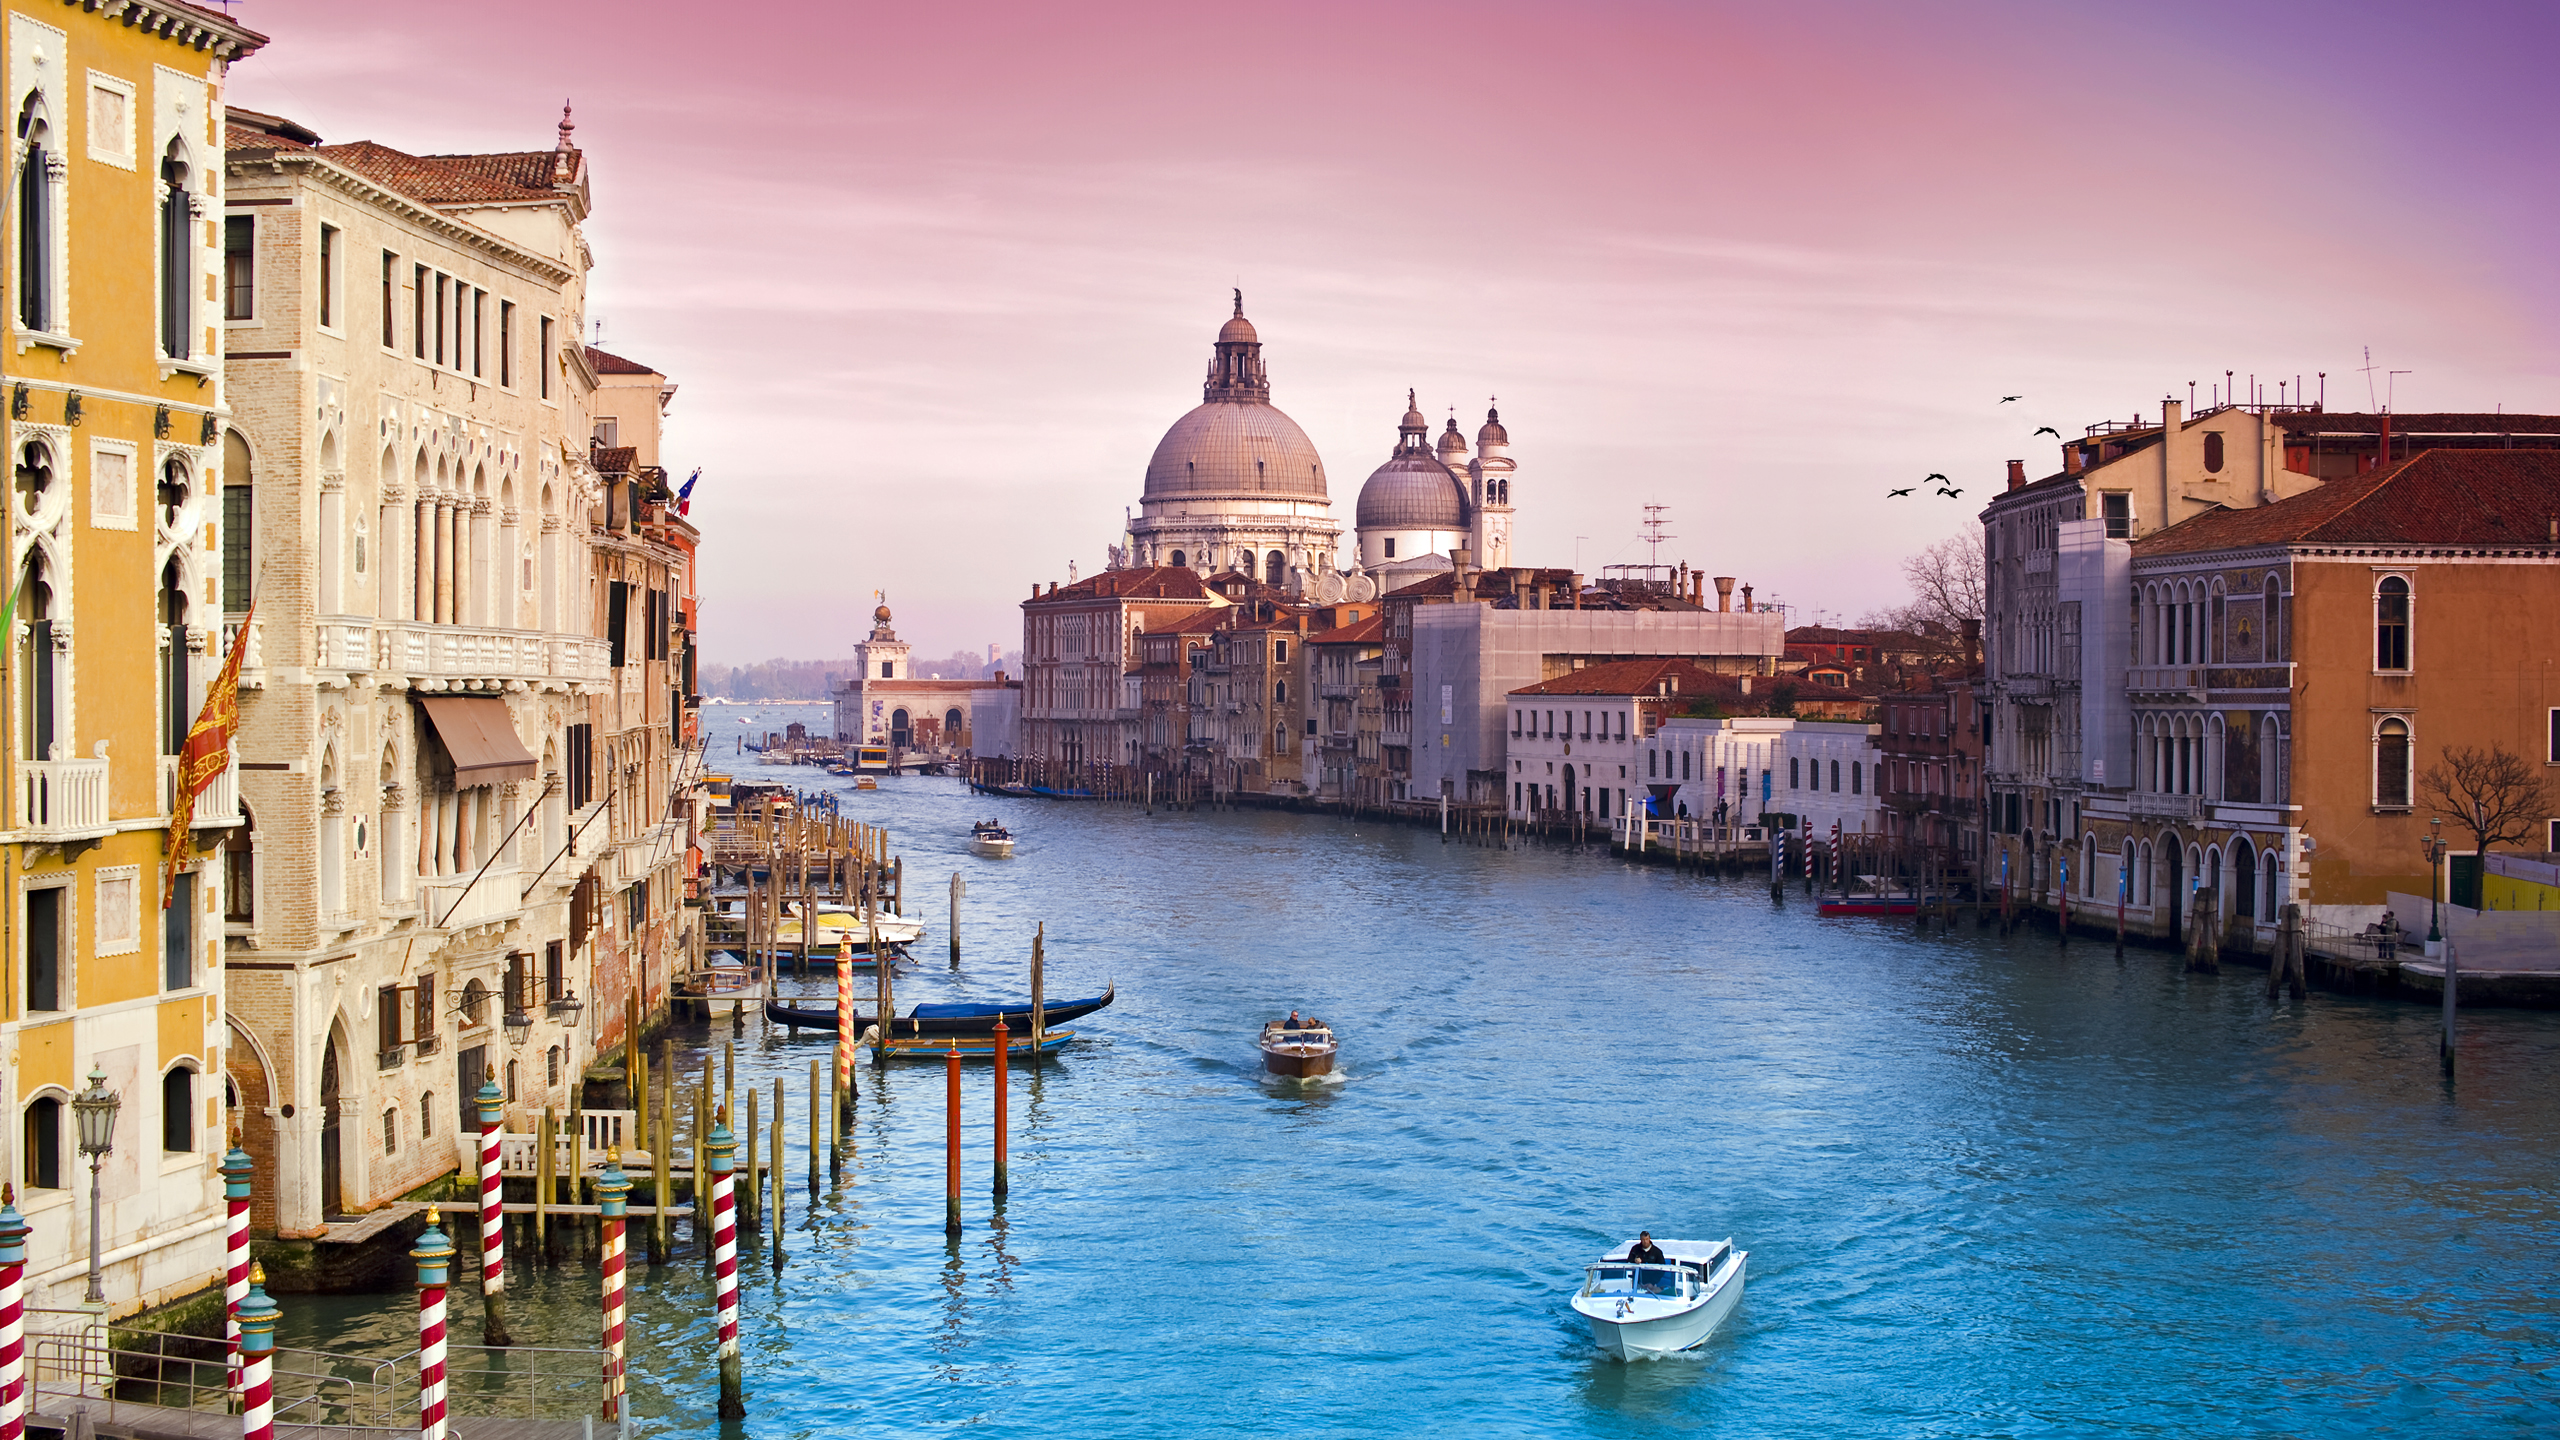
\includegraphics[width = 16cm]{im.jpg}
		\caption{Vestibulum euismod dictum elit. Nunc sed ex magna. Integer sed sapien rutrum, pellentesque odio nec, maximus ex}
		\label{fig:my_label}
	\end{center}
\end{figure}


Quisque cursus orci quam, non fermentum nisl dictum sed. Mauris accumsan feugiat lacus sed luctus. Proin tristique porttitor consectetur. Proin laoreet sagittis orci. Praesent iaculis at enim at eleifend. Nullam in quam cursus nibh mattis accumsan. Mauris quis nunc vestibulum, accumsan sapien ac, malesuada est~\cite{Adelson_Velskiy,MEI-1}. Donec nec nisl vitae mi rutrum tempus vel a urna. Donec a cursus neque, accumsan dictum erat. Sed rutrum, odio ac consequat efficitur, erat elit pulvinar justo, eget cursus augue neque a nulla. Donec dapibus a magna nec mollis. Maecenas tellus elit, tristique sit amet finibus eu, viverra at mi. Donec scelerisque consectetur nulla non congue.

\begin{center}
	\begin{table}[h]
		\caption{Donec in hendrerit libero, at efficitur arcu. Sed vestibulum facilisis diam.}
		\label{goodCatOrNot}
		\centering
		\begin{tabular}{|l|l|l|l|}
			\hline
			Mauris sagittis &  Malesuada libero & Sed rutrum diam volutpat & Vestibulum ante ipsum \\
			\hline
			Ultrices	&  8 & 146.77 & Primis\\ 
			\hline
			Posuere cubilia	& 6 & 358.65 & Luctus \\ 
			\hline
			Curae	&  3 & 799.39 & Faucibus \\ 
			\hline
		\end{tabular}
	\end{table}
\end{center}

Nam felis augue~\ref*{goodCatOrNot}, imperdiet sit amet eros ac, fermentum cursus nibh. Aenean in justo eu odio fermentum hendrerit eget at nibh. Ut lorem ex, tempor vitae viverra malesuada, suscipit pulvinar diam. Sed in odio felis. Morbi sed diam dictum, efficitur ipsum vehicula, rutrum orci. Nam consectetur eleifend est, ac maximus sem maximus in. In nec turpis massa. Nullam non erat sed nisi ultrices posuere eget vel ante. Aliquam sapien enim, vehicula sed nisl eget, vestibulum imperdiet dui. Duis et felis massa. Fusce et faucibus neque. 
\newpage\chapter{Sed eget tincidunt orci}

Nunc leo sem, tincidunt quis condimentum nec, suscipit id purus. Vivamus massa magna, eleifend at sollicitudin id, auctor vehicula dolor. Integer lectus dui, porta eget euismod eu, lacinia a est. Donec velit nibh, facilisis ut feugiat dictum, porta vestibulum sem. Ut tincidunt tortor congue consequat pellentesque. Sed maximus augue at gravida aliquam. Integer ex felis, porttitor a vehicula nec, scelerisque et leo. Sed nunc massa, laoreet a interdum ut, posuere mattis dolor. Integer consectetur, velit nec auctor rutrum, sem urna dignissim justo, nec venenatis elit augue eu sem.
\section{Ut malesuada nisi sit amet ornare aliquet}
Mauris vitae turpis maximus nibh suscipit bibendum quis in mauris. Morbi dolor arcu, lacinia vitae dolor at, condimentum blandit dui. Ut dictum arcu ac eros consequat aliquet. Nam id neque arcu. Donec molestie urna a massa sodales, ut dictum turpis tincidunt. Nunc fringilla vitae orci sit amet viverra. Cras eu lacus tempus, vestibulum nisl id, ultricies nisi. Integer quis lobortis velit. In ultrices diam et eros imperdiet congue. Proin quis dolor venenatis, tincidunt turpis in, porta tortor. Sed sit amet ipsum arcu. Nulla facilisi~\cite{Bocharnkinov_Ukraine}. Nam euismod nisl at elit gravida, at consectetur mauris commodo.

Ut varius vehicula tempus. Etiam at aliquam purus. Lorem ipsum dolor sit amet, consectetur adipiscing elit. Curabitur euismod diam libero, nec convallis leo placerat nec. Pellentesque habitant morbi tristique senectus et netus et malesuada fames ac turpis egestas. Proin nisl tortor, placerat vitae vestibulum eget, placerat consectetur nulla. Nullam at venenatis augue. Mauris sit amet dignissim urna, at efficitur nisl. Vestibulum cursus mattis quam, ac placerat purus dictum id. Nunc ut nulla sed elit facilisis feugiat.
\section{In et convallis velit, vel placerat ligula}
Morbi auctor scelerisque molestie. Duis dui nisi, scelerisque ut lacus vitae, accumsan faucibus tellus. Vestibulum pellentesque tempor orci eget venenatis. Suspendisse consequat lorem lorem, ac aliquam libero ultricies nec. Cras nec bibendum ipsum. Fusce feugiat nisi nec risus facilisis, eu congue nibh vehicula. Fusce efficitur magna a mi volutpat, et varius purus mattis. Aliquam erat volutpat. Pellentesque hendrerit vehicula turpis, imperdiet mattis turpis congue id. Phasellus mollis laoreet nisl in dignissim~\ref{fig:my_label2}. In pulvinar pellentesque nibh. Nullam condimentum porta ligula non volutpat.

\begin{figure}[H]
	\begin{center}
		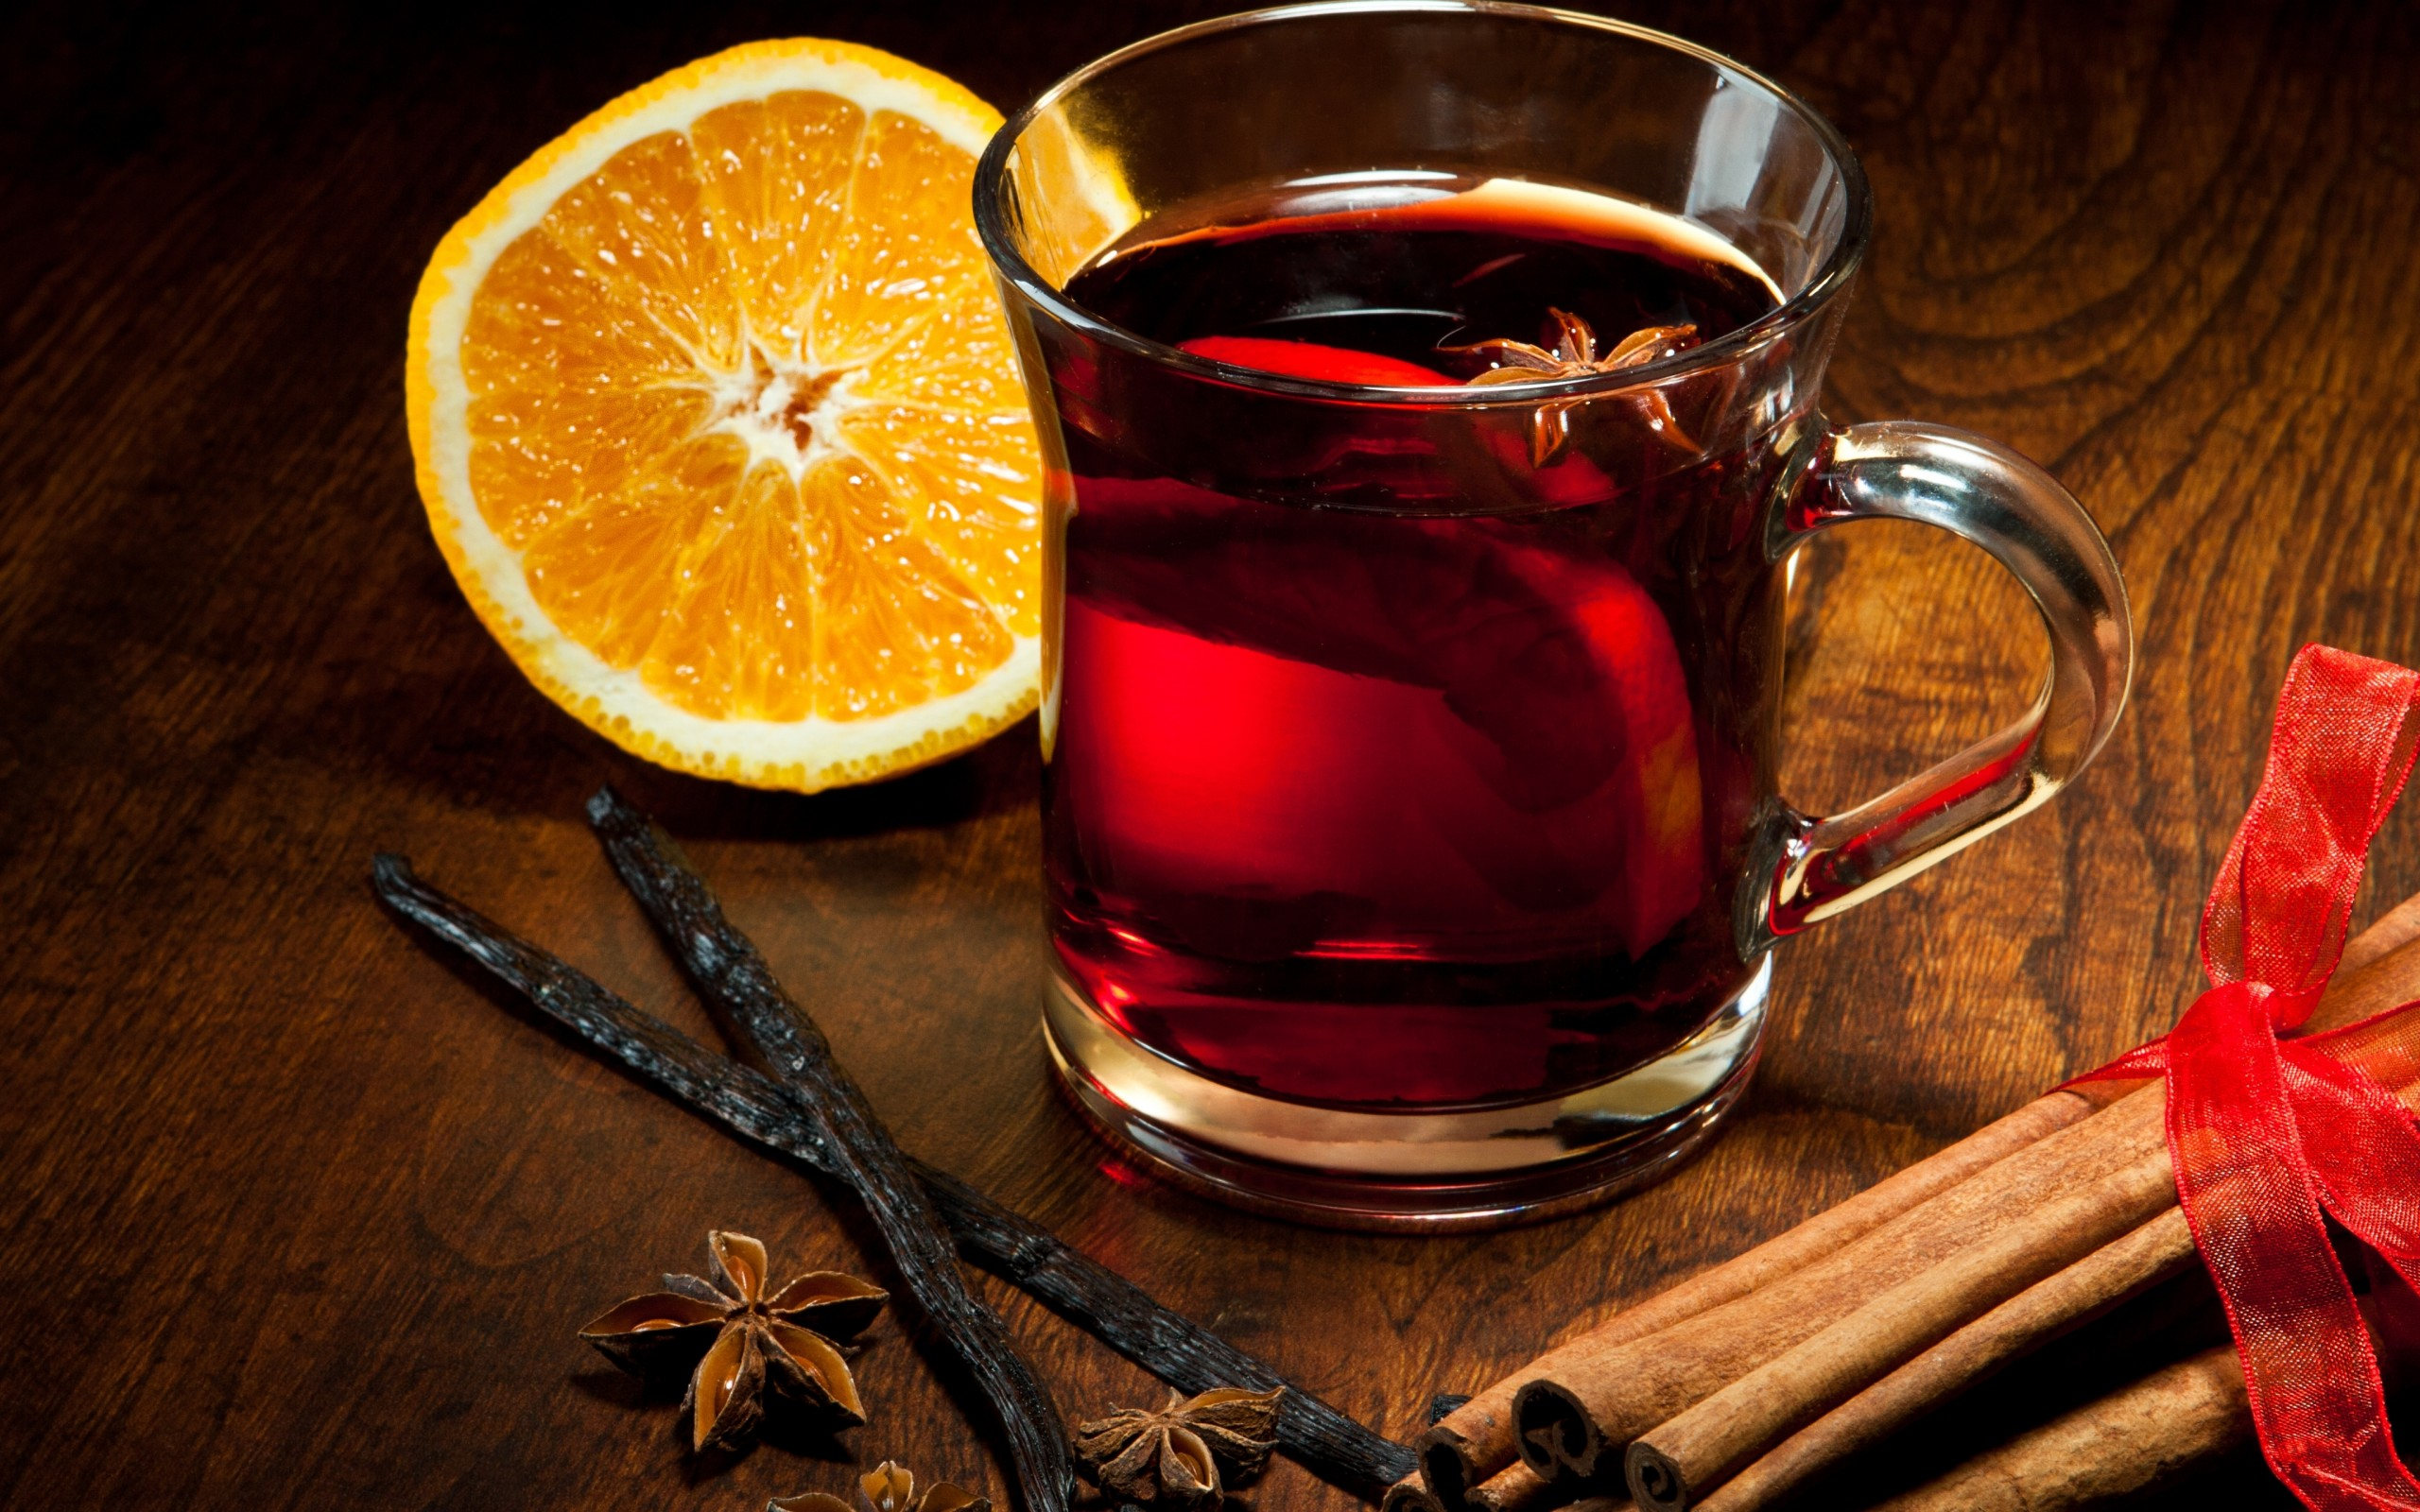
\includegraphics[width = 16cm]{im2.jpg}
		\caption{Vestibulum congue volutpat velit vel facilisis}
		\label{fig:my_label2}
	\end{center}
\end{figure}

Nam ac pellentesque tellus. Fusce cursus ultrices varius. Aenean imperdiet ipsum est, ut efficitur libero sagittis quis. Maecenas rutrum, sem sit amet condimentum pretium, massa tellus ornare mi, id dictum diam mauris quis dui. Integer vitae justo ex. Proin vitae suscipit orci, in lacinia nibh. Morbi nec tortor id elit sollicitudin sodales. Aenean bibendum scelerisque sagittis. Cras sit amet porttitor mauris, non facilisis urna.

Proin orci mi, ultricies non tellus at, consequat commodo massa. Curabitur id tincidunt libero, a tristique quam. Vestibulum vestibulum eros felis. Class aptent taciti sociosqu ad litora torquent per conubia nostra, per inceptos himenaeos. Maecenas non risus nec leo porttitor scelerisque. In consequat mauris sed imperdiet accumsan. Lorem ipsum dolor sit amet, consectetur adipiscing elit. Nullam eu luctus odio. Morbi vel gravida turpis. Suspendisse at est neque.
\section{Etiam nec quam aliquam, semper sapien sit amet, egestas ante}
Praesent rutrum at nibh quis posuere. In egestas, enim quis vehicula pharetra, orci massa scelerisque quam, nec semper est enim a enim. Nam eu auctor justo. Mauris iaculis, dolor eu lacinia imperdiet, mauris metus lobortis diam, id tempor sem dui nec sem. Vivamus enim dolor, pulvinar ac eleifend ut, pretium non nisl. Sed non auctor sapien, vitae blandit mauris. Proin porttitor lorem quis arcu blandit fermentum. Maecenas et massa ac felis mattis porta in sit amet elit~\cite{PhD_Starodubtsev,ivankov2014}. Aenean eu molestie enim. Maecenas sodales nisi sit amet sapien luctus consequat. Aliquam nec congue nulla. Morbi tincidunt nibh ipsum.
 

\newpage
\bibliographystyle{ugost2008}%% стилевой файл для оформления по ГОСТу 
\bibliography{ref}     %% имя библиографической базы (bib-файла) 

\newpage\clearpage
\likechapter{Приложение}
\section*{Приложение А}
\addcontentsline{toc}{section}{Приложение А}
Integer eget mauris lacinia, porttitor velit suscipit, fermentum purus. Aenean sed lorem elit. Pellentesque habitant morbi tristique senectus et netus et malesuada fames ac turpis egestas. Class aptent taciti sociosqu ad litora torquent per conubia nostra, per inceptos himenaeos. In aliquet ex et tortor accumsan, ut pharetra justo tincidunt. Vestibulum id dolor ac dolor vestibulum imperdiet a sit amet tellus. Aliquam et leo justo. Morbi at dui facilisis, aliquam magna a, lobortis turpis. Pellentesque sit amet egestas sem, eget accumsan lacus.
~\\
~\\
\textbf{Nam ornare vitae eros in mollis}:
\lstinputlisting[language=Matlab, basicstyle=\cyrillicfonttt\footnotesize ]{listings/Find3NN.m} 
~\\ 

\end{document}
